\chapter{SYSTEM ANALYSIS}
 
 \section{Module Description}
 The College Event Management System is divided into multiple functional modules, each playing a key role in ensuring smooth operations, secure access, and an engaging user experience. The main modules include:
 \begin{itemize}
    \item \textbf{User Authentication \& RBAC Module:} This module is responsible for handling user registrations, logins, and strict Role-Based Access Control (RBAC). It ensures that users are authenticated and routed to their respective dashboards based on their assigned roles: Super Admin, Admin/Faculty, or Student. It secures the application by preventing unauthorized access to administrative functions.
    \item \textbf{Event Management Module:} This is the core module used primarily by administrators and faculty. It allows for the dynamic creation, editing, deleting, and categorization of college events. It includes advanced features such as setting \texttt{max\_participants} capacity limits and managing an \texttt{approval\_status} workflow for events proposed by students.
    \item \textbf{Registration Module:} This module manages student participation in approved events. It allows students to RSVP to events while strictly enforcing capacity limits to prevent overbooking. Furthermore, it incorporates backend logic to prevent duplicate signups by the same student for a single event, ensuring fair opportunity and accurate participant tracking.
    \item \textbf{Dashboard \& Analytics Module:} This module provides role-specific visual interfaces. For Administrators and Faculty, it offers an analytics-driven dashboard to monitor event statistics, registration numbers, and pending approvals. For Students, it provides a personalized overview displaying their upcoming registered events and the status of events they have proposed.
    \item \textbf{Category Management Module:} Event categorization is managed here, allowing events to be grouped by taxonomical sorting (e.g., Arts, Sports, Cultural, Technical). This module powers the filtering functionality on the frontend, making it easier for students to discover events aligned with their interests.
    \item \textbf{UI \& Interaction Module:} The user interface ensures a professional and responsive experience across all devices. Built using Tailwind CSS, this module manages layouts, sidebar navigation, clear typography, and micro-interactions like hover states and transitions, creating an intuitive and modern workflow for all stakeholders.
\end{itemize}

\section{Business Rules}
Business rules are specific guidelines, conditions, or constraints that govern the operations of a business or system. They define how processes and activities should be conducted to ensure consistency, fairness, and alignment with business objectives.\\\\
\textbf{Event Creation and Approval}
\begin{itemize}
    \item Only Super Admins and Admin/Faculty members can directly publish active events to the platform.
    \item Students are allowed to propose new events, but these fall into a "Pending" state and must be explicitly approved by an Admin/Faculty member before becoming visible for registration.
    \item Every event must be assigned a specific category to facilitate system-wide filtering.
\end{itemize}
\textbf{Registration Mechanics}
\begin{itemize}
    \item Students can only register for events that are in an "Approved" or "Active" state.
    \item The system must enforce the \texttt{max\_participants} limit. Once the capacity is reached, no further registrations are permitted for that specific event.
    \item A single student account cannot register for the same event more than once.
\end{itemize}
\textbf{User Role Constraints}
\begin{itemize}
    \item The Super Admin role bypasses certain restrictions and holds full system access, including overarching analytics and system-wide configuration.
    \item Admin/Faculty users are restricted to event management, approval workflows, and administrative reporting, but cannot alter core system parameters.
    \item Student accounts are restricted to front-end browsing, registration actions, and tracking their own personal activity.
\end{itemize}

\newpage
\section{Analysis of Architecture (and/ or) Algorithms}
{\large \textbf{Laravel Framework \& MVC Architecture}}\\\\
The project is built on Laravel 11, a robust PHP framework renowned for its elegant syntax and developer-friendly tools. It utilizes the Model-View-Controller (MVC) architectural pattern to strictly separate business logic from presentation, ensuring maintainability and scalability.\\\\
\begin{enumerate}
    \item \textbf{Model (Database \& Core Logic):}
    \begin{itemize}
        \item Eloquent ORM is used to interact with the database using object-oriented syntax. Models such as User, Event, and Registration define the data structures and relationships.
        \item Database Migrations and Seeders are utilized to create structured tables and populate the system with initial test data iteratively.
    \end{itemize}
    \item \textbf{View (User Interface):}
    \begin{itemize}
        \item Laravel's Blade templating engine is combined with Tailwind CSS to generate dynamic, responsive HTML pages.
        \item Views are logically separated into distinct layouts for Admins and Students to ensure tailored user experiences.
    \end{itemize}
    \item \textbf{Controller (Request Handling):}
    \begin{itemize}
        \item Controllers act as the intermediary between Models and Views. They process incoming HTTP requests, apply business logic (like capacity checks), and return the appropriate views or JSON responses.
    \end{itemize}
    \item \textbf{Routing and Middleware:}
    \begin{itemize}
        \item Laravel's routing engine maps URLs to specific controller actions. 
        \item Middleware is heavily applied to enforce RBAC, ensuring that unauthorized users are redirected before they can access restricted routes or execute unauthorized actions.
    \end{itemize}
\end{enumerate}
\textbf{Why Laravel for College Event Management?}\\\\
Laravel provides a comprehensive web development framework that ensures high security, particularly regarding authentication, session handling, and database interactions. Its built-in tools like Artisan, Eloquent, and Blade significantly accelerate the development pipeline while maintaining a clean, highly structured codebase perfectly suited for institutional software.

\section{Project Pipeline}
\begin{figure}[H]
    \centering
    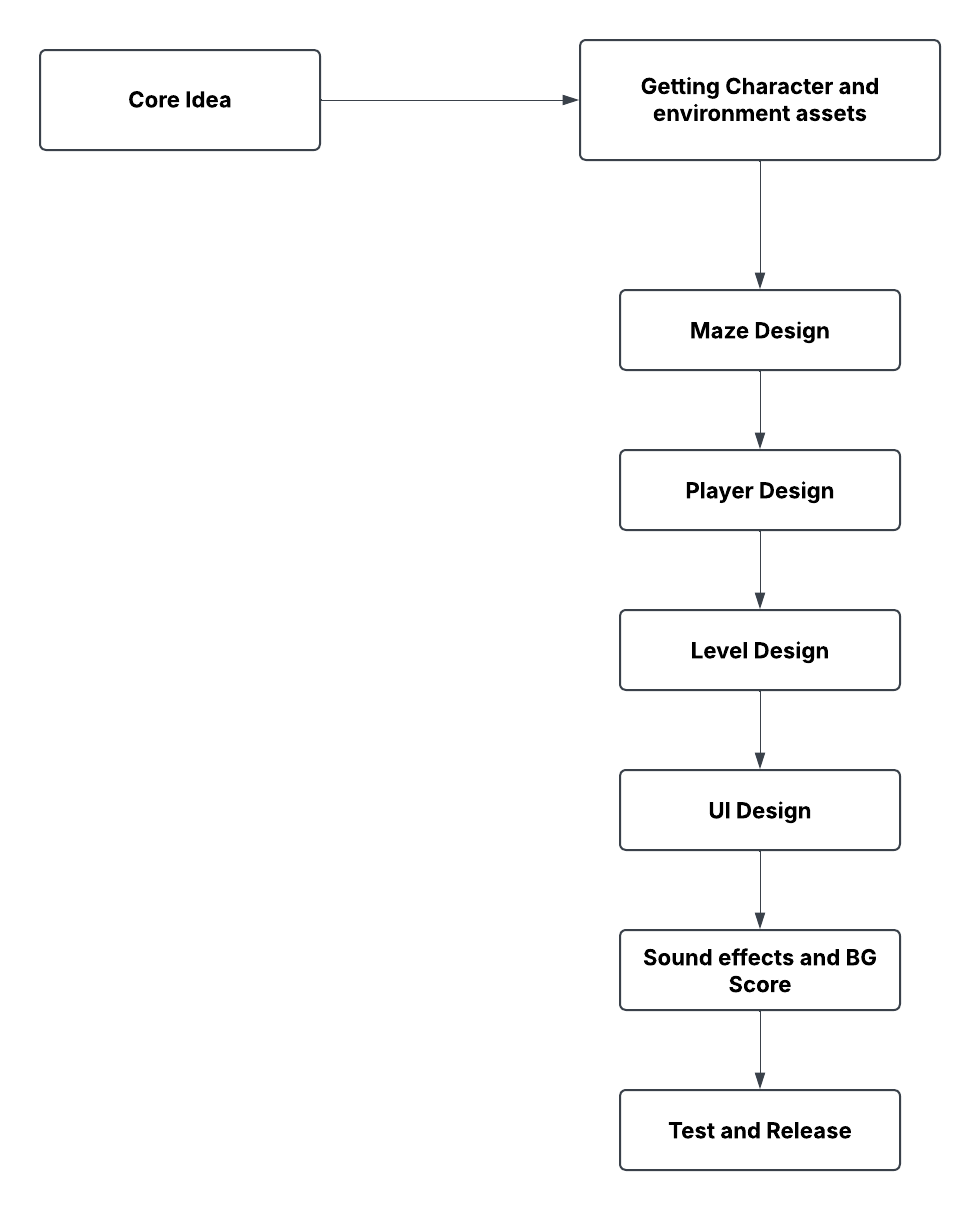
\includegraphics[width=1\textwidth]{project_pipe.png}
    \caption{Project Pipeline}
    \label{fig:project_pipeline}
\end{figure}

 \section{Feasibility Analysis}
 
 \subsection{Technical Feasibility}
 Technical feasibility assesses whether a project can be successfully developed and implemented using the current available technology, skills, and resources.\\\\
 \noindent
The technologies chosen for the College Event Management System are highly feasible and represent industry standards for modern web development. The backend utilizes PHP 8.2+ and the Laravel 11 framework, which provides built-in, secure authentication via Laravel Breeze, routing, and ORM. The frontend leverages Tailwind CSS, allowing for rapid UI development without writing complex custom CSS, compiled efficiently using Vite. The database architecture relies on a standard relational database (MySQL/PostgreSQL), easily managed via Laravel migrations. Development tools like Composer and Node.js/NPM ensure streamlined dependency management. The MVC architecture ensures that the system is scalable and easily maintainable, making it an excellent technical fit for the project’s objectives.

 \subsection{Economical Feasibility}
 Economic feasibility refers to the assessment of the financial aspects of a project to determine whether it is cost-effective and viable.\\\\
 The economic feasibility of the College Event Management System is highly favorable. The core technologies—PHP, Laravel, Node.js, Tailwind CSS, and MySQL—are entirely open-source and free to use. There are no proprietary software licensing fees required to build or host the core application logic. Local development is completely free using tools like XAMPP or Laravel Sail. Furthermore, the application is designed to be lightweight and can be easily deployed on affordable shared hosting or cloud VPS providers. By digitalizing the event management process, the system reduces the administrative overhead and paper waste associated with traditional management methods, providing long-term cost savings for the institution.
 
 \subsection{Operational Feasibility}
 Operational feasibility evaluates whether the project aligns with operational requirements and whether it can be smoothly integrated into existing processes.\\\\
 The operational feasibility of this system is strong because it directly addresses the pain points of manual college event organization. By centralizing event discovery, approval workflows, and registrations, it replaces fragmented processes (like spreadsheets and paper flyers) with a unified digital platform. The intuitive interfaces designed for distinct roles (Super Admin, Faculty, Student) require minimal training. System-enforced capacity limits and automatic duplicate-prevention eliminate manual administrative checking. Because the application is web-based and responsive, students and faculty can access it easily from any device without installing dedicated software, ensuring high adoption rates and smooth integration into the daily operational life of the college.

 \section{System Environment}
 
 \subsection{Software Environment}
 \textbf{Backend Framework: Laravel 11 (PHP 8.2+)}\\
 The core backend logic, routing, database interactions (Eloquent ORM), and authentication are handled by Laravel 11 running on PHP 8.2 or higher.\\\\
 \textbf{Frontend Styling: Tailwind CSS \& Blade}\\
 The user interfaces are constructed using Laravel's native Blade templating engine, heavily styled using the utility-first Tailwind CSS framework to ensure custom, responsive layouts.\\\\
 \textbf{Authentication \& Scaffolding: Laravel Breeze}\\
 Laravel Breeze is utilized for providing an immediate, secure, and robust starting point for implementing login, registration, password reset, and dashboard structures.\\\\
 \textbf{Build Tools: Vite \& Node.js}\\
 Node.js and NPM are utilized to manage frontend packages, while Vite serves as the modern, lightning-fast frontend build tool to compile Tailwind CSS and JavaScript assets.\\\\
 \textbf{Database Management: MySQL / MariaDB}\\
 A relational database management system is used to persistently store all user data, event details, registration logs, and categories securely.
 
 \subsection{Hardware Environment}
 \textbf{Processor (CPU):} Minimum dual-core processor (i3/Ryzen 3) or higher.\\\\
 \textbf{Memory (RAM):} 8 GB or higher.\\\\
 \textbf{Storage:} 256 GB SSD (Minimal space required for the application, varies based on database size and uploaded media).\\\\
 \textbf{Operating System:} Windows 10/11, macOS, or Linux (Ubuntu).
 \newpage
 
 \section{Actors and roles}
 The system involves three primary actors: Super Admin, Admin/Faculty, and Student.\\\\
\noindent
\textbf{Actors Name: Super Admin}
\\\\
 \textbf{Role:}
 \begin{itemize}
    \item Possesses full system access, bypassing most standard restrictions.
    \item Capable of viewing overarching administrative analytics and performing system-wide audits.
    \item Manages high-level configurations and user role assignments if necessary.
\end{itemize}

\noindent
\textbf{Actors Name: Admin / Faculty}
\\\\
\textbf{Role:}
\begin{itemize}
    \item Acts as the primary organizer and moderator for college events.
    \item Creates, edits, deletes, and monitors events and their capacities.
    \item Reviews and approves or rejects event proposals submitted by students.
    \item Accesses analytics dashboards to track event registrations and engagement.
\end{itemize}

\noindent
\textbf{Actors Name: Student}
\\\\
\textbf{Role:}
\begin{itemize}
    \item The end-user of the system, interacting through a personalized dashboard.
    \item Browses available active events and filters them by category.
    \item Registers (RSVPs) for events up to the predefined capacity limit.
    \item Can propose new events which are sent to the administrative backlog for approval.
    \item Views and manages their own active registrations and activity history.
\end{itemize}
